\chapter{The Experiment}
\label{cha:exper}

\section{Setup}

\subsection{Hardware}

All the tests were conducted on a laptop with a commodity processor
(Intel\textregistered Core\texttrademark $\,i5$ at $2.40$GHz). In
order to enforce serial execution, in case low level libraries attempted multi-threading \footnote{We are talking about BLAS 
  or LAPACK; as the high level algorithms used were serial.}, we used
the Linux  
\emph{taskset} command. The laptop has $8$Gb of RAM, but no more than 512Mb
were used on each experiment (and only for dense matrix algorithms;
sparse ones used much less). \\

\subsection{Software}

The implementations of the algorithms we used, were basically Python
wrappers against native libraries. These packages were SciPy
\cite{scipy} and NetworkX \cite{networkx}. On the other hand, the
native libraries actually offering the algorithm implementations were:

\begin{itemize}
  \item LAPACK \cite{lapack}, which provides (among many other things)
    the \gls{MRRR} implementation. LAPACK is actually the industrial
    standard for dense matrix computations. LAPACK is implemented in
    Fortran90 \footnote{At least the opensource version we used, as
      there are other commercial implementations as well.}.

  \item ARPACK \cite{arpack}, which provides the variant of the
    Lanczos algorithm that we tested (\gls{IRLM}). It also relies on LAPACK
    as a lower layer. ARPACK is implemented in Fortran77.

  \item Scipy \cite{scipy}, which delivers the implementation of
    \gls{LOBPCG} that we tested. While Scipy may also use LAPACK for several
    lower level operations, is interesting that \gls{LOBPCG} is the only
    algorithm that is implemented in Python. This makes reading its
    code a much easier task, than say, reading the Fortran77 ARPACK. 
\end{itemize}

As it can be perceived, all the algorithm implementations ultimately
rely on LAPACK; and this in turn, relies on BLAS \cite{blas}. All
those libraries were installed on the laptop, of course. The
\gls{SCC} algorithm mentioned in \cref{sub:avoid-clust-eigv} is
also offered by the Scipy package 
\footnote{The routine is
  \emph{scipy.sparse.csgraph.connected\_component}}. Last but not 
least, same SciPy also provides the sparse formats we tested (CSR and CSC). \\

Overall, Scipy makes quite accessible a lot of scientific
software; it feels like a new generation MATLAB that is becoming more
and more popular \footnote{A new competitor entered the arena
  recently, the Julia Programming Language (see \cite{julia}); which
  was specifically
  designed for scientific computing. We tried this language as well,
  for some of the experiments; but ended up preferring the maturity
  and wider repertoire of the Python + SciPy combo.}. Another merit of Scipy,
is that its performance is quite close to that of native code (we
also tested calling the libraries, like ARPACK, from low level C
code). The little penalty in performance by using the Python wrappers,
is definitely worth it in terms of development productivity. 

\section{Data Preparation}

\subsection{The actual data}
We created 10 random matrices from application's domain data, using
the same encoding techniques they use in production. The sizes of such
matrices are in the range $[867,4500]$, so they fit in memory without
problem. \\

\subsection{Sparse formats}
Two sparse matrix formats were tested with \gls{IRLM} and
\gls{LOBPCG} 
algorithms; namely the Compressed Sparse Row (CSR) and Compressed
Sparse Column (CSC) formats. For an overview of these and related
formats, in the actual context where we experimented with them, the
reader can consult \cite{johansson15}. While both formats showed
similar performance results, we prefer CSR because is the proper
format to use with the \gls{ClusteredEigenvalues} removal pre-processing (see
\cref{sub:avoid-clust-eigv} below). 

\subsection{Avoiding \gls{ClusteredEigenvalues}}
\label{sub:avoid-clust-eigv}

As we mentioned on previous chapter, \gls{ClusteredEigenvalues} were a
headache for both \gls{IRLM} and \gls{LOBPCG}; so we needed to do something
about them. By researching deeper why they were occurring, we found
that graphs behind the \gls{Laplacian}s produced by the
application, presented a common pattern: a disconnected graph with an
small component (2-3 nodes), and a big component (the rest of the
nodes). \\

The theory says that for a disconnected graph of two components, the
first and second eigenvalues of the \gls{Laplacian} will be zero (see
\cite{luxburg07}). In practice, what you get instead are two very
small numbers; and that is an extreme case of clustered
eigenvalues. They are very close to each other, because both try to
approximate zero. \\

The solution for this issue was to simply remove the already
disconnected small component; this makes sense given that ultimately,
the high level operation we want to perform on the graph is a
bi-partition (thus, expectation is that the graph is connected). The
caveat was to compute the Strongly Connected Components (\gls{SCC}) and the
new weights matrix quite efficiently, such that this pre-processing
did not become a performance penalty. The \gls{SCC} computation can be done
efficiently (sub-second) with algorithm documented in \cite{pearce05},
for which we did not dig its internals but just used the
implementation available in SciPy. This  
algorithm/implementation actually, is the reason why we prefer CSR
format over CSC (if the weights matrix is not passed in CSR format,
the routine takes much more time). \\

\newpage
The re-computation of the weights matrix $W$ though, required bit more
of thought. It turned out that the CSR format is not very friendly
with row/column removal operations (which we need to do, in order to
simulate that nodes got removed from the graph). Based on an
StackOverflow post \cite{alim15}, we took the idea of using an
intermediate sparse sparse format (COO) which allows for faster
column/row removals; but at the same time, it also allows for fast CSR
conversion. The current StackOverflow post has an even faster option
published now\footnote{This comment was written on 2016-08-25.}, but the
Python code below was good enough for our experiments: 

    \begin{lstlisting}
def split_cc_sparse2(W, cclab):
    idx_del = np.nonzero(cclab)[0]
    keep_row = np.logical_not(np.in1d(W.row, idx_del))
    keep_col = np.logical_not(np.in1d(W.col, idx_del))
    keep = np.logical_and(keep_row, keep_col)
    W.data = W.data[keep]
    W.row = W.row[keep]
    W.col = W.col[keep]
    W.row -= np.less.outer(idx_del, W.row).sum(0)
    W.col -= np.less.outer(idx_del, W.col).sum(0)
    k = len(idx_del)
    W._shape = (W.shape[0] - k, W.shape[1] - k)
    return W
    \end{lstlisting}
    \joinbelow{1cm}
    
The snippet above works as follows: the argument
\emph{cclab} contains the node labels for the components, namely $0$ and $1$,
for the big and small components respectively. Our goal is to
eliminate the nodes with 
label $1$ from the weights matrix $W$. For that, that lines $2-8$
begin by shrinking the index and data arrays (after removal of unwanted
columns/rows); then lines $9-10$ eliminate the potential gaps on the
indices and finally lines $11-12$ truncate the $W$ matrix to the new
size. The key idea is to do all the operations in terms of the NumPy
\cite{numpy} array primitives, which are quite efficient. \\

The overall pre-processing to eliminate the \gls{ClusteredEigenvalues} 
showed an average time of $1.2$ secs for the biggest
matrices, this includes: the \gls{SCC} computation, the routine above
to calculate new weights matrix, its conversion from COO
to CSR format and the recalculation of the \gls{Laplacian}. \\

There is an alternate approach (at least for \gls{LOBPCG}), that we
did not explore but that is worth mentioning (as it comes from Knyazev
himself, the creator of \gls{LOBPCG}). Rather tha pre-processing the
graphs to remove the disconnected component, one could simply
increase the $k$ (see \cref{sub:lobpcg}) to something not less than
the size of the eigenvalues cluster (which  
seems 2 or 3 for our application). It will be interesting to 
explore that option, and see how it compares in execution time
with our current approach. Actually, a comment by Strang in
\cite{strang88} (when talking about the convergence of the ``Block
Power Method'' \footnote{A version of the Power Method that can
  approximate several eigenvectors.}), suggests that this may
also help \gls{IRLM};this is 
just a quick thought, further research will be needed to confirm
it. We did not have time to explore these ideas, but they could be part of
a follow up of this thesis.

\subsection{Shifting the spectra}

The \gls{Cholmod} linear solver (\cite{cholmod08},
  \cite{cholmod08a}) mentioned on \cref{sub:irlm}, requires
that the matrix is Symmetric Positive Definite; and the \gls{Laplacian} is
not (it is symmetric, but has
one zero eigenvalue). Doing a little shift on the eigenvalues ($L +
0.01I$), makes the \gls{Laplacian} Positive-Definite as required. At the
end of the algorithm execution, we can just subtract the same shift from
the obtained eigenvalue to get the actual answer (which is not really
that relevant, as we mostly want the eigenvector; the eigenvalues are
just side products that the algorithms also produce). 

\section{Results}

Though the laptop was idle at the time of the experiments, we captured
run times as averages out of 100 executions (for each
algorithm/matrix combination); this was done with the intention of
removing the noise generated by background processes and other factors
which may affect the experiment. The graph below shows the results
obtained by encoding the matrices in CSR format. We present a
two-dimensional graph, with the X-axis representing the matrix size
and the Y-axis the average execution time in seconds. 

\begin{figure}[H]
  \centering
  \caption{Experiment Results in CSR format}  
  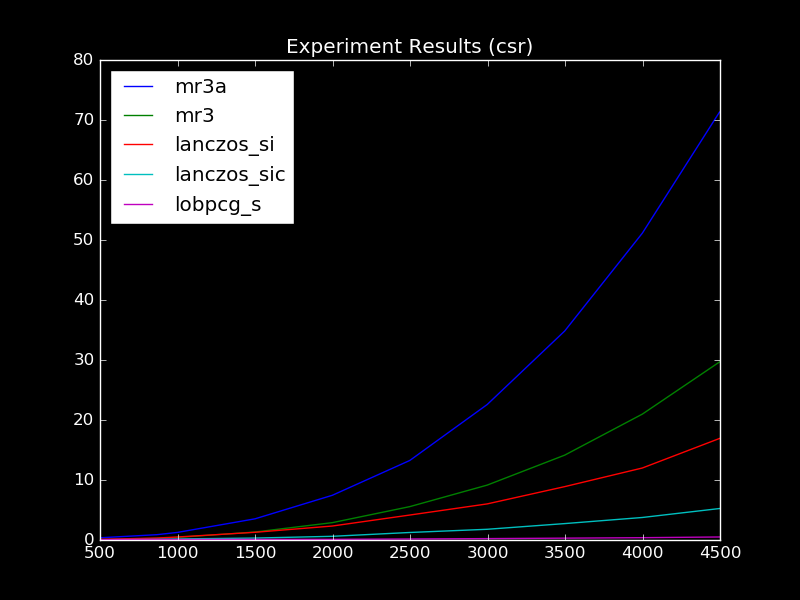
\includegraphics[width=11cm,height=8cm]{results-csr}
\end{figure}

Let us review each line in more detail (we talk mainly about the times
for the biggest matrix):

\begin{itemize}
\item The green line (label \emph{mr3a}) represents the times for the
  \gls{MRRR} algorithm, for 
  computing all the eigenpairs. This is not exactly the same time
  the application will get today, as the algorithm is different; but
  it could be considered as a lower bound (given that \gls{MRRR} is the
  state of the art for dense matrices). We can see that the time for
  the biggest matrix goes a bit higher than 70 seconds.
\item The blue line (label \emph{mr3}) is also the \gls{MRRR} algorithm, but
  taking advantage of its main feature \footnote{From the perspective
    of our problem, as the literature may consider other features of
    the algorithm as more relevant in a general context.}: the
  ability to compute in 
  isolation just the eigenpair we need. We can see that doing so,
  reduces the time to a bit less than 30 seconds (for the biggest
  matrix).
\item The orange line (label \emph{lanczos\_si}) is the first sparse
  matrix algorithm; it consists in the Lanczos variant \gls{IRLM}
  using \gls{SuperLU} 
  as the linear solver. Even when such solver is not specialized for
  the \gls{Laplacian} matrix, it can reduce the time to a bit less than 20
  seconds.
  \item The sky blue line (label \emph{lanczos\_sic}) is the very same
    \gls{IRLM} algorithm, but this time using the \gls{Cholmod} linear solver. We
    can see that using a more specialized solver, that is optimized
    for Symmetric Positive Definite matrices, pays off; to biggest
    time goes down to 5 seconds, approximately.
  \item The Lanczos variant \gls{IRLM}, combined with \gls{Cholmod} linear
    solver, was going to be our best time; until we discovered how to
    avoid the exceptions that the \gls{LOBPCG} implementation was raising, on
    the presence of \gls{ClusteredEigenvalues} (see
    \cref{sub:avoid-clust-eigv}). That brought this purple 
    line (label \emph{lobpcg\_s}), which by far beats them all; the time
    goes into sub-second scale even for the biggest matrix (the actual
    average time is around half a second, sometimes a bit bigger but
    still within a second). This makes \gls{LOBPCG} the definite winner of
    the experiment. 
\end{itemize}

Even with an apparent idle laptop,
  and with \emph{taskset} command, there were still variations on the
  average times; a more precise mechanism could be to boot the laptop
  into an special mode where there are less admin tasks running on the
background. This was not considered critical for our experiment, as
the pattern in the execution times was consistent; only difference was
a shift of the whole pattern (but \gls{LOBPCG} times remained in sub-second
scale). \\ 

Putting aside the fluctuations mentioned above; the CSC results are
basically the same than the CSR ones. A sample execution is shown
below: 

\begin{figure}[H]
  \centering
  \caption{Experiment Results in CSC format}   
  \includegraphics[width=11cm,height=8cm]{results-csc}
\end{figure}

Even when both formats behave well with the sparse algorithms, we
prefer CSR for reasons explained already on this chapter (see
\cref{sub:avoid-clust-eigv}). 

\section{Why \gls{LOBPCG} beats \gls{IRLM}?}
\label{sec:why-lobpcg}

The dramatic advantage that \gls{LOBPCG} shows against
Lanczos/\gls{IRLM} calls for our attention, and for an attempt to
explain why it occurred. We will do so based on the theory presented
in \cref{cha:algs}. The \cref{tab:lanczos-vs-lobpcg} summarizes all
the advangates 
that we see in \gls{LOBPCG} over Lanczos/\gls{IRLM}; and the rest of
this section will detail each point.

\begin{table}[h]  
  \caption{Lanczos(IRLM) vs LOBPCG}\label{tab:lanczos-vs-lobpcg}
  \begin{tabular}{l | c | c | }
    Feature/Issue & Lanczos(IRLM) & LOBPCG (single) \\
    \hline \hline
    Need Restarting &
    Yes, due $\Krylov{\inv{L}}{\vec{x}_0}{m}$ &
    No, $\func{span} \{\vec{x}_i, T\vec{r}_i, \vec{x}_{i-1}\}$ \\
    \hline
    Search strategy &
    Plain search &
    $\nabla (\func{\rho}(\vec{x_i}))$ \\
    &
    &
    $\suchthat \vec{r}_i = L\vec{x}_i - \func{\rho}(\vec{x}_i)\vec{x}_i$\\
    \hline
    Search Constraints &
    No &
    Yes ($\ortc{Y} = \ortc{\vec{1}}$) \\
    \hline
    Requested spectra &
    $k=2$ &
    $k=1$ \\      
    \hline
    Matrix operation &
    solve $L\vec{x} = \vec{b}$ &
    $L\vec{x}$ \\
    \hline      
    Uses Preconditioning &
    Only with iter solvers &
    Yes $\left(T = \dfrac{1}{\func{diag}(L)} \right)$ \\
    \hline
    Clustered eigenvalues &
    Inherited from PM &
    Bug? \\      
    \hline
  \end{tabular}
\end{table}

\subsection{No need for restarting}

Given that \gls{LOBPCG} uses a fixed-size generator set for the
searching-subspace, $\func{span} \{\vec{x}_i, T\vec{r}_i,
\vec{x}_{i-1}\}$, it does not need to invest extra time ensuring the
size remains low. This is contrary to \gls{IRLM}, which needs to
ensure the dimension of $\Krylov{\inv{L}}{\vec{x}_0}{m}$ does not grow
too much (causing unbounded memory consumption).

\subsection{Clever search strategy}

While \gls{IRLM} does not seem to follow a particular search strategy,
\gls{LOBPCG} leverages the gradient of the Rayleigh-Quotient, $\nabla
(\func{\rho}(\vec{x_i}))$, on each iteration.

\subsection{Search constrains / Requested spectra}

\gls{LOBPCG} can focus on searching for the smallest eigenpair (see
\cref{sub:lobpcg}), while \gls{IRLM} needs to compute the first and the
second. This is because the former offers the capability to restrict
the search to the orthogonal space $\ortc{Y}$ \footnote{Where matrix
  $Y$ is passed as input.}, which fits perfectly our use case (we set
$\ortc{Y} = \ortc{\vec{1}}$, as $\vec{1}$ is the first known
eigenvector of the \gls{Laplacian}; associated with its smallest
eigenvalue zero).

\subsection{Cheaper iterations}

One of the main goals in the design of \gls{LOBPCG} (see
\cite{knyazev01}, \cite{knyazev03}),
was to be as cheap as the regular \footnote{Regular means here, that
  we use
  the algorithm to compute the biggest eigenpairs; as opposed to the
  use of the shift-invert-mode, which aims to compute the opposite
  side of the spectra.} invocation of Lanczos
algorithms (like \gls{IRLM}), which only involves a matrix
multiplication ($L\vec{x}$) per iteration; and this goal was achieved
indeed. This contrasts with the far heavier operation that \gls{IRLM}
needs to address on each iteration, when called in shift-invert mode;
namely to solve the linear system $L\vec{x} = \vec{b}$.  


\subsection{Use of preconditioner}

The \gls{IRLM} algorithm only allows for preconditioners in the
sub-problem of solving the linear system $L\vec{x} = \vec{b}$, when we
opt to use iterative solvers instead of direct-methods \footnote{The deal
  here, is that direct methods are forbidden for huge matrices; which
  fortunately was not our case, as they fit just fine in memory.}. But
unless those linear solvers are used to compute high accuracy
answers (which may not be easy with an iterative solver), they could
slow down overall  convergence of \gls{IRLM} (see \cite{knyazev03}). The
situation is different for \gls{LOBPCG}, which considers a preconditioner $T$ for
the eigensolver itself. It is an optional argument, but we found that using
it significantly speeds up the execution times. The preconditioner
used , $T = \dfrac{1}{\func{diag}(L)} $, was taken from NetworkX
package \cite{networkx}.

\subsection{Clustered eigenvalues}

This is perhaps the only point where we may declare a tie; as both
implementations have issues with \gls{ClusteredEigenvalues}. But
\gls{LOBPCG} still seems to show an advantage here; as it does not
inherit (at least not directly), the slow convergence that \gls{IRLM}
gets from the Power Method. Instead, the implementation of
\gls{LOBPCG} seems to rather have a defect (exception risen on the
presence of \gls{ClusteredEigenvalues}).

